% Options for packages loaded elsewhere
\PassOptionsToPackage{unicode}{hyperref}
\PassOptionsToPackage{hyphens}{url}
\PassOptionsToPackage{dvipsnames,svgnames,x11names}{xcolor}
%
\documentclass[
  letterpaper,
  DIV=11,
  oneside]{scrreprt}

\usepackage{amsmath,amssymb}
\usepackage{iftex}
\ifPDFTeX
  \usepackage[T1]{fontenc}
  \usepackage[utf8]{inputenc}
  \usepackage{textcomp} % provide euro and other symbols
\else % if luatex or xetex
  \usepackage{unicode-math}
  \defaultfontfeatures{Scale=MatchLowercase}
  \defaultfontfeatures[\rmfamily]{Ligatures=TeX,Scale=1}
\fi
\usepackage{lmodern}
\ifPDFTeX\else  
    % xetex/luatex font selection
\fi
% Use upquote if available, for straight quotes in verbatim environments
\IfFileExists{upquote.sty}{\usepackage{upquote}}{}
\IfFileExists{microtype.sty}{% use microtype if available
  \usepackage[]{microtype}
  \UseMicrotypeSet[protrusion]{basicmath} % disable protrusion for tt fonts
}{}
\makeatletter
\@ifundefined{KOMAClassName}{% if non-KOMA class
  \IfFileExists{parskip.sty}{%
    \usepackage{parskip}
  }{% else
    \setlength{\parindent}{0pt}
    \setlength{\parskip}{6pt plus 2pt minus 1pt}}
}{% if KOMA class
  \KOMAoptions{parskip=half}}
\makeatother
\usepackage{xcolor}
\usepackage[left=1in,marginparwidth=2.0666666666667in,textwidth=4.1333333333333in,marginparsep=0.3in]{geometry}
\setlength{\emergencystretch}{3em} % prevent overfull lines
\setcounter{secnumdepth}{5}
% Make \paragraph and \subparagraph free-standing
\ifx\paragraph\undefined\else
  \let\oldparagraph\paragraph
  \renewcommand{\paragraph}[1]{\oldparagraph{#1}\mbox{}}
\fi
\ifx\subparagraph\undefined\else
  \let\oldsubparagraph\subparagraph
  \renewcommand{\subparagraph}[1]{\oldsubparagraph{#1}\mbox{}}
\fi

\usepackage{color}
\usepackage{fancyvrb}
\newcommand{\VerbBar}{|}
\newcommand{\VERB}{\Verb[commandchars=\\\{\}]}
\DefineVerbatimEnvironment{Highlighting}{Verbatim}{commandchars=\\\{\}}
% Add ',fontsize=\small' for more characters per line
\usepackage{framed}
\definecolor{shadecolor}{RGB}{241,243,245}
\newenvironment{Shaded}{\begin{snugshade}}{\end{snugshade}}
\newcommand{\AlertTok}[1]{\textcolor[rgb]{0.68,0.00,0.00}{#1}}
\newcommand{\AnnotationTok}[1]{\textcolor[rgb]{0.37,0.37,0.37}{#1}}
\newcommand{\AttributeTok}[1]{\textcolor[rgb]{0.40,0.45,0.13}{#1}}
\newcommand{\BaseNTok}[1]{\textcolor[rgb]{0.68,0.00,0.00}{#1}}
\newcommand{\BuiltInTok}[1]{\textcolor[rgb]{0.00,0.23,0.31}{#1}}
\newcommand{\CharTok}[1]{\textcolor[rgb]{0.13,0.47,0.30}{#1}}
\newcommand{\CommentTok}[1]{\textcolor[rgb]{0.37,0.37,0.37}{#1}}
\newcommand{\CommentVarTok}[1]{\textcolor[rgb]{0.37,0.37,0.37}{\textit{#1}}}
\newcommand{\ConstantTok}[1]{\textcolor[rgb]{0.56,0.35,0.01}{#1}}
\newcommand{\ControlFlowTok}[1]{\textcolor[rgb]{0.00,0.23,0.31}{#1}}
\newcommand{\DataTypeTok}[1]{\textcolor[rgb]{0.68,0.00,0.00}{#1}}
\newcommand{\DecValTok}[1]{\textcolor[rgb]{0.68,0.00,0.00}{#1}}
\newcommand{\DocumentationTok}[1]{\textcolor[rgb]{0.37,0.37,0.37}{\textit{#1}}}
\newcommand{\ErrorTok}[1]{\textcolor[rgb]{0.68,0.00,0.00}{#1}}
\newcommand{\ExtensionTok}[1]{\textcolor[rgb]{0.00,0.23,0.31}{#1}}
\newcommand{\FloatTok}[1]{\textcolor[rgb]{0.68,0.00,0.00}{#1}}
\newcommand{\FunctionTok}[1]{\textcolor[rgb]{0.28,0.35,0.67}{#1}}
\newcommand{\ImportTok}[1]{\textcolor[rgb]{0.00,0.46,0.62}{#1}}
\newcommand{\InformationTok}[1]{\textcolor[rgb]{0.37,0.37,0.37}{#1}}
\newcommand{\KeywordTok}[1]{\textcolor[rgb]{0.00,0.23,0.31}{#1}}
\newcommand{\NormalTok}[1]{\textcolor[rgb]{0.00,0.23,0.31}{#1}}
\newcommand{\OperatorTok}[1]{\textcolor[rgb]{0.37,0.37,0.37}{#1}}
\newcommand{\OtherTok}[1]{\textcolor[rgb]{0.00,0.23,0.31}{#1}}
\newcommand{\PreprocessorTok}[1]{\textcolor[rgb]{0.68,0.00,0.00}{#1}}
\newcommand{\RegionMarkerTok}[1]{\textcolor[rgb]{0.00,0.23,0.31}{#1}}
\newcommand{\SpecialCharTok}[1]{\textcolor[rgb]{0.37,0.37,0.37}{#1}}
\newcommand{\SpecialStringTok}[1]{\textcolor[rgb]{0.13,0.47,0.30}{#1}}
\newcommand{\StringTok}[1]{\textcolor[rgb]{0.13,0.47,0.30}{#1}}
\newcommand{\VariableTok}[1]{\textcolor[rgb]{0.07,0.07,0.07}{#1}}
\newcommand{\VerbatimStringTok}[1]{\textcolor[rgb]{0.13,0.47,0.30}{#1}}
\newcommand{\WarningTok}[1]{\textcolor[rgb]{0.37,0.37,0.37}{\textit{#1}}}

\providecommand{\tightlist}{%
  \setlength{\itemsep}{0pt}\setlength{\parskip}{0pt}}\usepackage{longtable,booktabs,array}
\usepackage{calc} % for calculating minipage widths
% Correct order of tables after \paragraph or \subparagraph
\usepackage{etoolbox}
\makeatletter
\patchcmd\longtable{\par}{\if@noskipsec\mbox{}\fi\par}{}{}
\makeatother
% Allow footnotes in longtable head/foot
\IfFileExists{footnotehyper.sty}{\usepackage{footnotehyper}}{\usepackage{footnote}}
\makesavenoteenv{longtable}
\usepackage{graphicx}
\makeatletter
\def\maxwidth{\ifdim\Gin@nat@width>\linewidth\linewidth\else\Gin@nat@width\fi}
\def\maxheight{\ifdim\Gin@nat@height>\textheight\textheight\else\Gin@nat@height\fi}
\makeatother
% Scale images if necessary, so that they will not overflow the page
% margins by default, and it is still possible to overwrite the defaults
% using explicit options in \includegraphics[width, height, ...]{}
\setkeys{Gin}{width=\maxwidth,height=\maxheight,keepaspectratio}
% Set default figure placement to htbp
\makeatletter
\def\fps@figure{htbp}
\makeatother
\newlength{\cslhangindent}
\setlength{\cslhangindent}{1.5em}
\newlength{\csllabelwidth}
\setlength{\csllabelwidth}{3em}
\newlength{\cslentryspacingunit} % times entry-spacing
\setlength{\cslentryspacingunit}{\parskip}
\newenvironment{CSLReferences}[2] % #1 hanging-ident, #2 entry spacing
 {% don't indent paragraphs
  \setlength{\parindent}{0pt}
  % turn on hanging indent if param 1 is 1
  \ifodd #1
  \let\oldpar\par
  \def\par{\hangindent=\cslhangindent\oldpar}
  \fi
  % set entry spacing
  \setlength{\parskip}{#2\cslentryspacingunit}
 }%
 {}
\usepackage{calc}
\newcommand{\CSLBlock}[1]{#1\hfill\break}
\newcommand{\CSLLeftMargin}[1]{\parbox[t]{\csllabelwidth}{#1}}
\newcommand{\CSLRightInline}[1]{\parbox[t]{\linewidth - \csllabelwidth}{#1}\break}
\newcommand{\CSLIndent}[1]{\hspace{\cslhangindent}#1}

\usepackage{booktabs}
\usepackage{longtable}
\usepackage{array}
\usepackage{multirow}
\usepackage{wrapfig}
\usepackage{float}
\usepackage{colortbl}
\usepackage{pdflscape}
\usepackage{tabu}
\usepackage{threeparttable}
\usepackage{threeparttablex}
\usepackage[normalem]{ulem}
\usepackage{makecell}
\usepackage{xcolor}
\usepackage{caption}
\KOMAoption{captions}{tableheading}
\makeatletter
\makeatother
\makeatletter
\@ifpackageloaded{bookmark}{}{\usepackage{bookmark}}
\makeatother
\makeatletter
\@ifpackageloaded{caption}{}{\usepackage{caption}}
\AtBeginDocument{%
\ifdefined\contentsname
  \renewcommand*\contentsname{Inhaltsverzeichnis}
\else
  \newcommand\contentsname{Inhaltsverzeichnis}
\fi
\ifdefined\listfigurename
  \renewcommand*\listfigurename{Abbildungsverzeichnis}
\else
  \newcommand\listfigurename{Abbildungsverzeichnis}
\fi
\ifdefined\listtablename
  \renewcommand*\listtablename{Tabellenverzeichnis}
\else
  \newcommand\listtablename{Tabellenverzeichnis}
\fi
\ifdefined\figurename
  \renewcommand*\figurename{Abbildung}
\else
  \newcommand\figurename{Abbildung}
\fi
\ifdefined\tablename
  \renewcommand*\tablename{Tabelle}
\else
  \newcommand\tablename{Tabelle}
\fi
}
\@ifpackageloaded{float}{}{\usepackage{float}}
\floatstyle{ruled}
\@ifundefined{c@chapter}{\newfloat{codelisting}{h}{lop}}{\newfloat{codelisting}{h}{lop}[chapter]}
\floatname{codelisting}{Listing}
\newcommand*\listoflistings{\listof{codelisting}{Listingverzeichnis}}
\makeatother
\makeatletter
\@ifpackageloaded{caption}{}{\usepackage{caption}}
\@ifpackageloaded{subcaption}{}{\usepackage{subcaption}}
\makeatother
\makeatletter
\@ifpackageloaded{tcolorbox}{}{\usepackage[skins,breakable]{tcolorbox}}
\makeatother
\makeatletter
\@ifundefined{shadecolor}{\definecolor{shadecolor}{rgb}{.97, .97, .97}}
\makeatother
\makeatletter
\makeatother
\makeatletter
\@ifpackageloaded{sidenotes}{}{\usepackage{sidenotes}}
\@ifpackageloaded{marginnote}{}{\usepackage{marginnote}}
\makeatother
\makeatletter
\makeatother
\ifLuaTeX
\usepackage[bidi=basic]{babel}
\else
\usepackage[bidi=default]{babel}
\fi
\babelprovide[main,import]{ngerman}
% get rid of language-specific shorthands (see #6817):
\let\LanguageShortHands\languageshorthands
\def\languageshorthands#1{}
\ifLuaTeX
  \usepackage{selnolig}  % disable illegal ligatures
\fi
\IfFileExists{bookmark.sty}{\usepackage{bookmark}}{\usepackage{hyperref}}
\IfFileExists{xurl.sty}{\usepackage{xurl}}{} % add URL line breaks if available
\urlstyle{same} % disable monospaced font for URLs
\hypersetup{
  pdftitle={Kausalanalyse und Machine Learning in R},
  pdfauthor={Martin C. Arnold, Christoph Hanck},
  pdflang={de},
  colorlinks=true,
  linkcolor={blue},
  filecolor={Maroon},
  citecolor={Blue},
  urlcolor={Blue},
  pdfcreator={LaTeX via pandoc}}

\title{Kausalanalyse und Machine Learning in R}
\usepackage{etoolbox}
\makeatletter
\providecommand{\subtitle}[1]{% add subtitle to \maketitle
  \apptocmd{\@title}{\par {\large #1 \par}}{}{}
}
\makeatother
\subtitle{Ein Leitfaden für reproduzierbare Forschung}
\author{Martin C. Arnold, Christoph Hanck}
\date{2022-11-01}

\begin{document}
\maketitle
\ifdefined\Shaded\renewenvironment{Shaded}{\begin{tcolorbox}[breakable, interior hidden, enhanced, sharp corners, boxrule=0pt, borderline west={3pt}{0pt}{shadecolor}, frame hidden]}{\end{tcolorbox}}\fi

\renewcommand*\contentsname{Inhaltsverzeichnis}
{
\hypersetup{linkcolor=}
\setcounter{tocdepth}{2}
\tableofcontents
}
\bookmarksetup{startatroot}

\hypertarget{einleitung}{%
\chapter*{Einleitung}\label{einleitung}}
\addcontentsline{toc}{chapter}{Einleitung}

\markboth{Einleitung}{Einleitung}

In den letzten Jahren hat sich die datengetriebene Forschung in vielen
Fachgebieten, insbesondere in der Ökonometrie und den empirischen
Wirtschaftswissenschaften, grundlegend verändert. Haupttreiber dieses
Wandels ist die zunehmende Verfügbarkeit von \emph{big data} --
hochdimensionale Datenmengen die regelmäßig in Unternehmen und
öffentlichen Institutionen anfallen und die Entwicklung sowie den
Einsatz neuer statistischer Verfahren im Gebiet \emph{machine learning}
prominent gemacht haben. Mit diesen Verfahren können große Datenmengen
schnell und effizient verarbeitet und analysiert werden, was ihre
zunehmende Relevanz für die evidenzbasierte Entscheidungsfindung in
Politik und Wirtschaft begründet.

Ein weiterer Treiber der empirischen wirtschaftswissenschaftlichen
Forschung ist die\footnote{Bekannst als \emph{the credibility revolution
  in empirical economics} (Angrist und Pischke 2010).}

\begin{itemize}
\item
  Data Science / Varian zitieren: der hat recht behalten
\item
  Reproducibility
\item
  Programmierung / Relevanz von Coding
\item
  kanonischer Unterrichtskatalog in Ökonometrie aufbrechen
\item
  Alles zusammenlegen als ein wichtiger Block für
  Wirtschaftswissenschaftler und solche die es werden wollen. Und es
  wird noch wichtiger werden.
\end{itemize}

(Angrist und Pischke 2010)

\bookmarksetup{startatroot}

\hypertarget{statistische-programmierung-mit-r}{%
\chapter{Statistische Programmierung mit
R}\label{statistische-programmierung-mit-r}}

Dieses Kapitel ist \emph{nicht} als umfassende Einführung in R gedacht,
sondern behandelt Kernkonzepte und soll der Selbsteinschätzung dienen.
Wenngleich die Inhalte deutlich über ein Hallo-Welt-Beispiel\footnote{https://de.wikipedia.org/wiki/Hallo-Welt-Programm}
hinausgehen, betrachten wir hier \textbf{absolutes Basiswissen}. Dieses
ist Vorraussetzung für das Verständnis fortgeschrittener Konzepte in
späteren Kapitel. Falls Sie bereits über solide Grundkenntnisse im
Umgang mit R verfügen, können Sie problemlos zu Kapitel XYZ springen.
Sollten Sie nicht oder nur teilweise mit den hier gezeigten Befehlen
vertraut sein, empfiehlt sich eine Erarbeitung bzw. Wiederholung der
Grundlagen. Nachstehede Ressourcen finden wir hilfreich:

\begin{itemize}
\item
  Feedbackgestütze interaktive Übungsaufgaben bei DataCamp, bspw.
  \href{https://campus.datacamp.com/courses/einfuhrung-in-r/}{Einführung
  in R}\footnote{Ein Teil des hier angebotenen Katalogs (exlusive
    \emph{Einführung in R}) ist kostenpflichtig.}
\item
  Open-source-Literatur wie der Umfangreiche Leitfaden von
  \href{https://methodenlehre.github.io/einfuehrung-in-R/}{Ellis und
  Mayer (2023)}.
\end{itemize}

Lorem ipsum dolor sit amet, consetetur sadipscing elitr, sed diam nonumy
eirmod tempor invidunt ut labore et dolore magna aliquyam erat, sed diam
voluptua. At vero eos et accusam et justo duo dolores et ea rebum. Stet
clita kasd gubergren, no sea takimata sanctus est Lorem ipsum dolor sit
amet. Lorem ipsum dolor sit amet, consetetur sadipscing elitr, sed diam
nonumy eirmod tempor invidunt ut labore et dolore magna aliquyam erat,
sed diam voluptua. At vero eos et accusam et justo duo dolores et ea
rebum. Stet clita kasd gubergren, no sea takimata sanctus est Lorem
ipsum dolor sit amet.

\hypertarget{pinguine-und-pipes}{%
\subsubsection{Pinguine und Pipes}\label{pinguine-und-pipes}}

\bookmarksetup{startatroot}

\hypertarget{regression-discontiniuty-designs}{%
\chapter{Regression Discontiniuty
Designs}\label{regression-discontiniuty-designs}}

Regression Discontinuity Design (RDD) ist ein Ansatz für die Schätzung
von Treatment-Effekten mit Regression, wenn durch einen experimentell
oder natürlich gegebenen Umstand die Behandlung an einem Schwellenwert
(\(C\)) einer \emph{Laufvariable} (\(X\)) sprunghaft beeinflusst wird.
Ein RDD-Schätzer brücksichtigt lediglich Beobachtungen mit Ausprägungen
von \(X\), die knapp ober- oder knapp unterhalb von \(C\) liegen. Die
zentrale Idee hierbei ist, dass Individuen nahe bei \(C\) im
Durchschnitt ähnliche Merkmale aufweisen. RDD isoliert Variation auf dem
Pfad \emph{Oberhalb C → Treatment → Y}. Somit können Backdoor-Pfade über
\(X\) oder weitere (möglichweise unbeobachtbare) Confounder (\(Z\))
vermieden werden, siehe Abbildung~\ref{fig-CDRDD}.

\begin{figure}

{\centering 

\begin{figure}[H]

{\centering 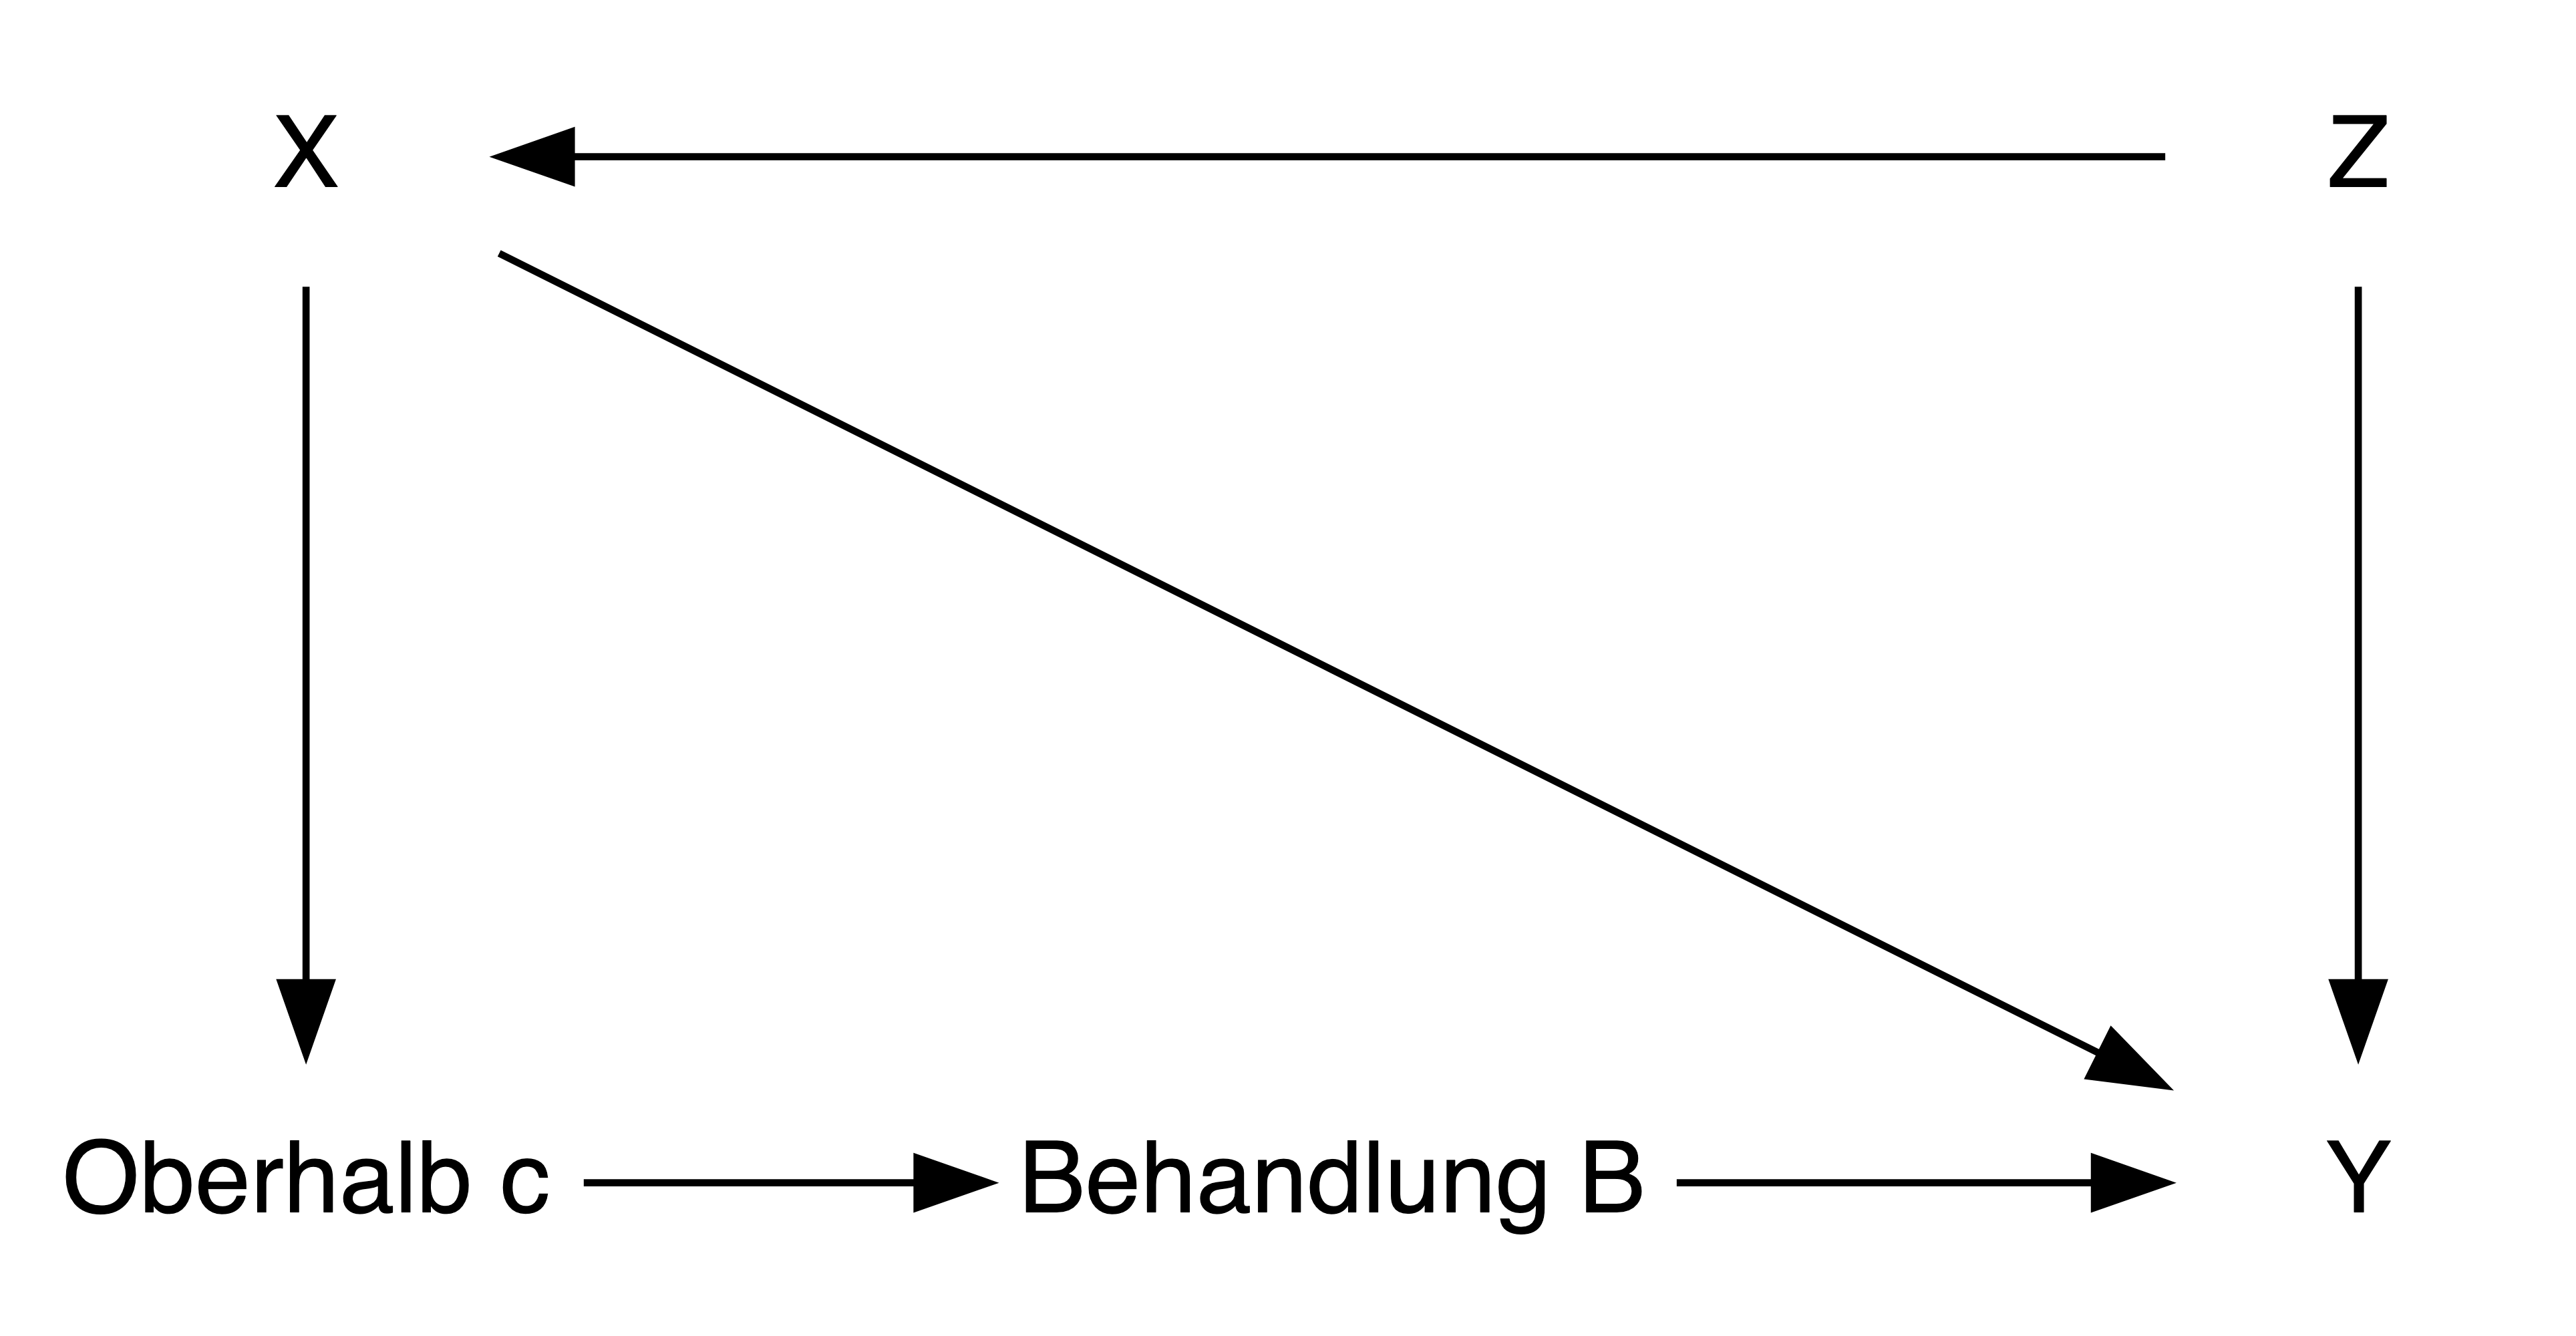
\includegraphics[width=5in,height=3in]{RDD_files/figure-latex/dot-figure-1.png}

}

\end{figure}

}

\caption{\label{fig-CDRDD}Causal Diagram für RDD}

\end{figure}

Der kausale Effekt wird dabei als durchschnittlicher Effekt der
Diskontinuität auf die Outcome-Variable (\(Y\)) anhand von Beobachtungen
\emph{nahe bei \(C\)} ermittelt.

Hinsichtlich der Beeinflussung der Behandlung unterscheiden wir zwischen
\emph{Sharp} und \emph{Fuzzy} Regression Discontinuity Designs
(SRDD/FRDD). Bei einem SRDD ist die Zuordnung \emph{deterministisch},
d.h. der Schwellenwert in der Laufvariable ist eine harte Grenze für die
Gruppenzugehörigkeit: Die \emph{Wahrscheinlichkeit} der Behandlung
springt bei \(X=C\) um \(p=100\%\).

Bei einem FRDD wird angenommen, dass die Zuordnung nicht perfekt durch
den Schwellenwert C bestimmt ist: Die \emph{Wahrscheinlichkeit} der
Behandlung springt bei \(X=C\) um \(p<100\%\).\footnote{Im FRDD können
  also sowohl Treatment- als auch Kontroll-Beobachtungen auf beiden
  Seiten der Diskontinuität beobachtet werden -- die Trennung der
  Gruppen ist ``unscharf'' (engl. \emph{fuzzy})} Dies tritt auf, wenn
das Überschreiten von \(C\) nicht die einzige Determinante einer
Behandlung ist. Die Wahl zwischen SRDD und FRDD hängt von der Natur der
Daten und der Forschungsfrage ab.

Der Geschätzte Treatment-Effekt ist ein s.g. \emph{local average
treatment effect} (LATE).

\hypertarget{sharp-regression-discontinuity-design}{%
\section{Sharp Regression Discontinuity
Design}\label{sharp-regression-discontinuity-design}}

\textbf{Modelle und funktionale Form}

Die korrekte Spezifikation der funktionalen Form für RDD ist wichtig, um
eine unverzerrte Schätzung des Effekts zu vermeiden. Die einfachste Form
eines SRDD kann anhand der linearen Regression \begin{align}
Y_i = \beta_0 + \beta_1 D_i + \beta_2 (X_i - C) + u_i\label{eq-simpleSRDD}
\end{align} geschätzt werden, wobei \(D_i\) Behandlung anzeigt: \(D_i\)
ist eine Dummy-Variable für das Überschreiten des Schwellenwertes C,
d.h. \begin{align*}
  D_i=\begin{cases}
    0 & X_i < C\\
    1 & X_i \geq C.
  \end{cases}
\end{align*} Hierbei ist zu beachten, dass \((X_i - C)\) die um den
Schwellenwert zentrierte Laufvariable ist, sodass \(\beta_1\) der Effekt
der Behandlung bei \((X_i - C)\geq 0\) ist.

Modell \eqref{eq-simpleSRDD} unterstellt, dass \(X\) links- und
rechtsseitig von \(C\) denselben Effekt \(\beta_2\) auf \(Y\) hat. Eine
Alternative ist ein lineares Interaktionsmodell \begin{align}
Y_i = \beta_0 + \beta_1 D_i + \beta_2 (X_i - C) + \beta_3(X_i-C)\times D_i + u_i.\label{eq:linearSRDD}
\end{align} In Modell \eqref{eq:linearSRDD} erfasst \(\beta_3\) den
Unterschied des Effekts von \(X\) auf \(Y\) für Beoabachtungen oberhalb
von \(C\) gegenüber Beobachtungen unterhalb von \(C\), sodass
unterschiedliche lineare Effekte von \(X\) auf \(Y\) link- und
rechtsseitig von \(C\) modelliert werden können.

\textbf{Bandweite}

Neben der funktionalen Form muss spezifiziert werden, welche
Beobachtungen hinreichend nahe am Schwellenwert C liegen. Hierfür
verwenden wir eine sogenannte Bandweite \(h\), wobei \begin{align}
  \lvert(X_i-C)\rvert\leq h \label{eq:bwc}
\end{align} das Kriterium für eine Berücksichtigung von Beobachtung
\(i\) bei der Schätzung ist. Unter Berücksichtigung einer Bandweite
\(h\) wird der Regressionsansatz \eqref{eq:linearSRDD} als \emph{local
linear regression} mit Uniform-Kernelfunktion bezeichnet.\footnote{\emph{Local
  regression} ist ein nicht-parametrisches Verfahren. Hierbei kann die
  Beziehung zwischen Variablen flexibel modelliert werden.} Der
Uniform-Kernel ist neben dem Triangular-Kernel eine häufig in der Praxis
genutzte lineare Kernelfunktion.\footnote{In der Praxis wird oftmals
  local linear regression mit linearen Kernelfunktionen zurückgegriffen
  und die Robustheit der Ergebnisse anhand flexiblerer Spezifikationen
  geprüft.} Der nachstehende Code plottet die Uniform- (grün) sowie die
Triangular-Kernelfunktion (blau) wie in Abbildung~\ref{fig-linearkern}
dargestellt.

\begin{Shaded}
\begin{Highlighting}[]
\FunctionTok{library}\NormalTok{(ggplot2)}
\FunctionTok{library}\NormalTok{(cowplot)}
\FunctionTok{ggplot}\NormalTok{() }\SpecialCharTok{+} 
    \FunctionTok{geom\_function}\NormalTok{(}
      \AttributeTok{fun =} \SpecialCharTok{\textasciitilde{}} \FunctionTok{ifelse}\NormalTok{(}\FunctionTok{abs}\NormalTok{(.) }\SpecialCharTok{\textless{}=} \DecValTok{1}\NormalTok{, }\DecValTok{1}\NormalTok{, }\DecValTok{0}\NormalTok{), }\AttributeTok{col =} \StringTok{"green"}
\NormalTok{      ) }\SpecialCharTok{+} 
    \FunctionTok{geom\_function}\NormalTok{(}
      \AttributeTok{fun =} \SpecialCharTok{\textasciitilde{}} \FunctionTok{ifelse}\NormalTok{(}\FunctionTok{abs}\NormalTok{(.) }\SpecialCharTok{\textless{}=} \DecValTok{1}\NormalTok{, }\DecValTok{1}\SpecialCharTok{{-}}\FunctionTok{abs}\NormalTok{(.), }\DecValTok{0}\NormalTok{), }\AttributeTok{col =} \StringTok{"blue"}
\NormalTok{      ) }\SpecialCharTok{+} 
    \FunctionTok{scale\_x\_continuous}\NormalTok{(}\StringTok{"x"}\NormalTok{, }\AttributeTok{limits =} \FunctionTok{c}\NormalTok{(}\SpecialCharTok{{-}}\FloatTok{1.5}\NormalTok{, }\FloatTok{1.5}\NormalTok{), }
                       \AttributeTok{labels =} \FunctionTok{c}\NormalTok{(}\StringTok{"{-}h"}\NormalTok{, }\DecValTok{0}\NormalTok{, }\StringTok{"h"}\NormalTok{), }
                       \AttributeTok{breaks =} \FunctionTok{c}\NormalTok{(}\SpecialCharTok{{-}}\DecValTok{1}\NormalTok{, }\DecValTok{0}\NormalTok{, }\DecValTok{1}\NormalTok{)) }\SpecialCharTok{+}
    \FunctionTok{scale\_y\_continuous}\NormalTok{(}\StringTok{"K(x)"}\NormalTok{, }
                       \AttributeTok{breaks =} \FunctionTok{c}\NormalTok{(}\DecValTok{0}\NormalTok{, }\DecValTok{1}\NormalTok{), }
                       \AttributeTok{limits =} \FunctionTok{c}\NormalTok{(}\DecValTok{0}\NormalTok{, }\FloatTok{1.5}\NormalTok{)) }\SpecialCharTok{+}
    \FunctionTok{theme\_cowplot}\NormalTok{()}
\end{Highlighting}
\end{Shaded}

\begin{marginfigure}

{\centering 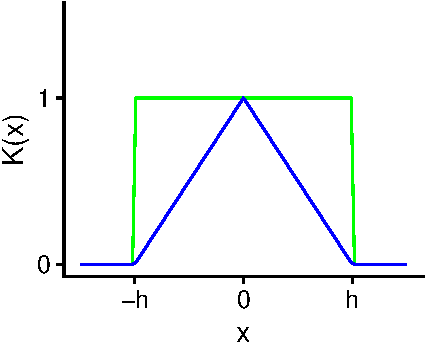
\includegraphics{RDD_files/figure-pdf/fig-linearkern-1.pdf}

}

\caption{\label{fig-linearkern}Uniform-Kernel auf {[}-h, h{]}}

\end{marginfigure}

Die Wahl der Bandweite ist eine wichtige Komponente der RDD-Schätzung.
Falls der wahre Zusammenhang nicht-linear ist, erlauben kleine
Bandweiten eine Schätzung der Regressionsfunktion nahe des
Schwellenwertes mit wenig Verzerrung. Allerdings kann diese Schätzung
unpräzise sein, wenn nur wenige Beobachtungen \eqref{eq:bwc} erfüllen.
In der Praxis wird \(h\) daher anhand einer Schätzfunktion (G. Imbens
und Kalyanaraman 2012) oder anhand von \emph{Cross Validation} (bspw. G.
W. Imbens und Lemieux 2008) bestimmt. Die später in diesem Kapitel
betrachteten R-Pakete halten diese Methoden bereit.

\hypertarget{beispiel-amtsinhaber-vorteil-lee2008}{%
\subsection{Beispiel: Amtsinhaber-Vorteil (Lee
2008)}\label{beispiel-amtsinhaber-vorteil-lee2008}}

Lee (2008) untersucht den Einfluss des Amtsinhaber-Vorteils auf die Wahl
von Mitgliedern des US-Repräsentantenhauses. Entfällt ein Stimmenanteil
von mehr als 50\% auf eine Partei, hat diese Partei den Vorsitz des
Repräsentantenhauses gewonnen. Durch die Analyse der 6558 Wahlen im
Zeitraum 1946-1998 mit RDD kommt die Studie zu dem Ergebnis, dass die
amtsinhabende im Durchschnitt einen Vorteil von etwa 8\%-10\% bei der
Wahl hat. Dieses Ergebnis kann als Vorteil kann durch verschiedene
Faktoren erklärt werden, bspw. dass die amtierende Partei höhere
finanzielle Ressourcen und von einer besseren Organisation als die
Opposition profitiert. Anhand der Datensätze \texttt{house} und
\texttt{house\_binned} illustrieren wir nachfolgend die Schätzung von
SRDD-Modellen für den Wahlerfolg der demokratischen Partei, wenn diese
Amtsinhaber ist.

Wir verschaffen uns zunächst einen Überblick über den Datensatz
\texttt{house}.

R lädt. Etwas Geduld bitte\ldots{}

\hypertarget{webr-editor-1}{}

\hypertarget{webr-code-output-1}{}

Der Datensatz \texttt{house} enthält Stimmenanteile der Demokraten bei
der Wahl zum Zeitpunkt \(T\) (\texttt{StimmenT}) sowie um den
Schwellenwert von 50\% zentrierte Stimmenanteile bei der vorherigen Wahl
zum Zeitpunkt \(T-1\) (\texttt{StimmenTm1}).

\texttt{house\_binned} ist eine aggregierte Version von \texttt{house}
mit Mittelwerten von jeweils 50 gleichgroßen Intervallen oberhalb und
unterhalb der Schwelle von 0. Dieser Datensatz eignet sich, um einen
ersten Eindruck des funktionalen Zusammenhangs auf beiden Seiten zu
gewinnen. Wir stellen die klassierten Daten mit \texttt{ggplot2}
graphisch dar.

R lädt. Etwas Geduld bitte\ldots{}

\hypertarget{webr-editor-2}{}

\hypertarget{webr-code-output-2}{}

Die Grafik zeigt eindeutig einen Sprung an der Stelle
\(StimmenTm1 = 0\). Weiterhin erkennen wir, dass der Zusammenhang nahe 0
jeweils gut durch eine lineare Funktion approximiert werden kann. Eine
Modell-Spezifikation mit gleicher Steigung auf beiden Seiten des
Schwellenwertes scheint hingegen ungeeignet.

Als nächstes fügen wir dem Datensatz eine Dummyvariable \texttt{D}
hinzu. Diese dient als Indikator für den Wahlgewinn in der letzten Wahl.

R lädt. Etwas Geduld bitte\ldots{}

\hypertarget{webr-editor-3}{}

\hypertarget{webr-code-output-3}{}

Als nächstes schätzen wir das Modell \begin{align}
  \text{StimmenT}_i = \beta_0 + \beta_1 D_i + \beta_2 (\text{StimmenTm1}_i - 50) + \beta_3(\text{StimmenTm1}_i - 50)\times D_i + u_i
\end{align} bei einer Bandweite von \(h = 1\). Aufgrund der Skalierung
der Daten bedeutet dies die Verwendung des \emph{gesamten} Datensatzes
für die Schätzung.

R lädt. Etwas Geduld bitte\ldots{}

\hypertarget{webr-editor-4}{}

\hypertarget{webr-code-output-4}{}

Der geschätzte Koeffizient von \(D\) (\texttt{DTRUE}) beträgt etwa 0.12
und ist hochsignifikant. Übereinstimmend mit der (oben erstellten)
Grafik erhalten wir also eine positive Schätzung des Treatment-Effekts.
Diese Schätzung könnte jedoch invalide sein:

\begin{itemize}
\item
  Die (implizite) Wahl von \(h=1\) macht die Isolation des relevanten
  Frontdoor-Paths (\(C=0\) → Treatment → StimmenT) wenig plausibel.
\item
  Weiterhin könnte die lineare funktionale Form unser Regression für den
  gesamten Datensatz inadäquat sein: Die lineare Approximation könnte
  lediglich ``lokal'' zu 0 gut sein und anderweitig in einer verzerrten
  Schätzung des Effekts resultieren.
\end{itemize}

\begin{Shaded}
\begin{Highlighting}[]
\FunctionTok{round}\NormalTok{(rdd}\SpecialCharTok{::}\FunctionTok{IKbandwidth}\NormalTok{(}\AttributeTok{X =}\NormalTok{ house}\SpecialCharTok{$}\NormalTok{StimmenTm1, }\AttributeTok{Y =}\NormalTok{ house}\SpecialCharTok{$}\NormalTok{StimmenT), }\AttributeTok{digits =} \DecValTok{4}\NormalTok{)}
\end{Highlighting}
\end{Shaded}

\begin{verbatim}
[1] 0.2685
\end{verbatim}

R lädt. Etwas Geduld bitte\ldots{}

\hypertarget{webr-editor-5}{}

\hypertarget{webr-code-output-5}{}

Die nachstehende interaktive Abbildung zeigt die klassierten Daten aus
Lee (2008) auf dem Intervall \([-0.5,0.5]\) gemeinsam mit einer
nicht-parametrischen Schätzung des Zusammenhangs von \texttt{StimmenT}
und \texttt{StimmenTm1} mit LOESS.\footnote{LOESS ist eine
  nicht-parametrische Regressionsmethode, die lokale Gewichte verwendet,
  um nicht-lineare Zusammenhänge zwischen Variablen zu modellieren und
  geglättete Funktionen anzupassen.} Über die Inputs kann eine
gemeinsame Bandweite \(l\in(0,1]\) für den LOESS-Schätzer auf beiden
Seiten des Schwellenwerts 0 und die Bandweite der Daten (\(h\)) um den
Schwellenwert angepasst werden. Beachte:

\begin{itemize}
\item
  Der geschätzte Zusammenhang ist etwa linear für die voreingestellten
  Parameter (\(l = 1\), \(h = 0.28\)).
\item
  Für kleine \(l\) passt sich die Schätzung Besser an die Datenpunkte
  an. Zu kleine Werte führen jedoch zu \emph{overfitting}. Insbesondere
  hat die geschätzte Funktion eine zu extreme Steigung nahe des
  Schwellenwerts → verzerrte Schätzung des Effekts!
\item
  Kleine Werte \(h\) bedeuten eine geringe Datenbasis, sodass LOESS
  selbst bei großen \(l\) zu nicht-linearen Anpassungen der
  Regressionsfunktion tendiert. Für solche Parameterkombinationen
  erfolgt die Schätzung des Effekts mit hoher Varianz.
\end{itemize}

\textbf{SRDD mit nicht-parametrischer Regression}

\begin{Shaded}
\begin{Highlighting}[]
\NormalTok{//| echo: false}
\NormalTok{html\textasciigrave{}}
\NormalTok{\textless{}style\textgreater{}}
\NormalTok{circle \{}
\NormalTok{  fill{-}opacity: .8;}
\NormalTok{  stroke: \#000;}
\NormalTok{  stroke{-}opacity: 1;}
\NormalTok{\}}
\NormalTok{.regression \{}
\NormalTok{  fill: none;}
\NormalTok{  stroke: \#000;}
\NormalTok{  stroke{-}width: 1.5px;}
\NormalTok{\}}
\NormalTok{.axis line \{}
\NormalTok{  stroke: \#ddd;}
\NormalTok{\}}
\NormalTok{.axis .baseline line \{}
\NormalTok{  stroke: \#555;}
\NormalTok{\}}
\NormalTok{.axis .domain \{}
\NormalTok{  display: none;}
\NormalTok{\} }
\NormalTok{\textless{}/style\textgreater{}}
\NormalTok{\textasciigrave{}}

\NormalTok{d3 = require("d3{-}array@3", "d3{-}axis@3", "d3{-}regression@1", "d3{-}scale@4", "d3{-}shape@3", "d3{-}selection@3")}

\NormalTok{margin = (\{left: 55, right: 8, top: 13, bottom: 24\});}
\NormalTok{base = Math.min(width, 500);}
\NormalTok{innerWidth = base {-} margin.left {-} margin.right;}
\NormalTok{innerHeight = base{-}100 {-} margin.top {-} margin.bottom;}

\NormalTok{viewof bandwidth = Inputs.range([.01, 1], \{}
\NormalTok{  label: "Bandweite LOESS (l)",}
\NormalTok{  step: .01,}
\NormalTok{  value: 1}
\NormalTok{\});}

\NormalTok{viewof bw\_daten = Inputs.range([.05, .5], \{}
\NormalTok{  label: "Bandweite Daten (h)",}
\NormalTok{  step: .01,}
\NormalTok{  value: .28}
\NormalTok{\});}

\NormalTok{xScaleLoess = d3.scaleLinear()}
\NormalTok{   .domain([{-}.55, .55])}
\NormalTok{   .range([0, innerWidth]);}
   
\NormalTok{yScaleLoess = d3.scaleLinear()}
\NormalTok{  .domain([.2, .8])}
\NormalTok{  .range([innerHeight, 0]);}

\NormalTok{lineLoess = d3.line()}
\NormalTok{  .x(d =\textgreater{} xScaleLoess(d[0]))}
\NormalTok{  .y(d =\textgreater{} yScaleLoess(d[1]));}
  
\NormalTok{xAxisLoess = d3.axisBottom(xScaleLoess)}
\NormalTok{  .tickSize(innerHeight + 10)}
\NormalTok{  .tickValues([{-}.5, {-}.25, 0, .25, .5])}
\NormalTok{  .tickFormat(d =\textgreater{} d);}

\NormalTok{yAxisLoess = d3.axisLeft(yScaleLoess)}
\NormalTok{  .tickSize(innerWidth + 10)}
\NormalTok{  .tickValues([.2, .35, .5, .65, .8])}
\NormalTok{  .tickFormat(d =\textgreater{} d);}

\NormalTok{loessRegression = d3.regressionLoess()}
\NormalTok{  .x(d =\textgreater{} d.StimmenTm1)}
\NormalTok{  .y(d =\textgreater{} d.StimmenT)}
\NormalTok{  .bandwidth(bandwidth);}
\end{Highlighting}
\end{Shaded}

\begin{Shaded}
\begin{Highlighting}[]
\NormalTok{//| echo: false}
\NormalTok{//| fig{-}cap: "Nicht{-}parametrische Regression auf beiden Seiten des Cut{-}offs."}

\NormalTok{\{}
\NormalTok{  const svg = d3.select(DOM.svg(innerWidth + margin.left + margin.right + 20, innerHeight + margin.top + margin.bottom + 20))}
  
\NormalTok{  const g = svg.append("g")}
\NormalTok{      .attr("transform", \textasciigrave{}translate($\{margin.left\}, $\{margin.top\})\textasciigrave{});}

\NormalTok{  g.append("g")}
\NormalTok{      .attr("class", "axis")}
\NormalTok{      .call(xAxisLoess);}

\NormalTok{  g.append("g")}
\NormalTok{    .attr("class", "axis")}
\NormalTok{    .attr("transform", \textasciigrave{}translate($\{innerWidth\})\textasciigrave{})}
\NormalTok{    .call(yAxisLoess);}

\NormalTok{  // Add X axis label:}
\NormalTok{  g.append("text")}
\NormalTok{    .attr("text{-}anchor", "end")}
\NormalTok{    .attr("font{-}size", 13)}
\NormalTok{    .attr("x", innerWidth)}
\NormalTok{    .attr("y", innerHeight + margin.top + 25)}
\NormalTok{    .text("Stimmenanteil Demokraten letzte Wahl");}

\NormalTok{  // Y axis label:}
\NormalTok{  g.append("text")}
\NormalTok{    .attr("text{-}anchor", "end")}
\NormalTok{    .attr("transform", "rotate({-}90)")}
\NormalTok{    .attr("font{-}size", 13)}
\NormalTok{    .attr("y", {-}margin.left+10)}
\NormalTok{    .attr("x", {-}margin.top+10)}
\NormalTok{    .text("Stimmenanteil Demokraten");}

\NormalTok{  // Distance at jump}
\NormalTok{  g.append("text")}
\NormalTok{   .attr("x", 250) // x{-}Position des Textelements}
\NormalTok{   .attr("y", 200) // y{-}Position des Textelements}
\NormalTok{   .text("") // Textinhalt}
\NormalTok{   .attr("font{-}size", "14px") // Schriftgröße}
\NormalTok{   .attr("fill", "black"); // Textfarbe}


\NormalTok{  g.selectAll("circle")}
\NormalTok{    .data(transpose(house\_binned))}
\NormalTok{    .enter().append("circle")}
\NormalTok{    .attr("r", 2)}
\NormalTok{    .attr("cx", d =\textgreater{} xScaleLoess(d.StimmenTm1))}
\NormalTok{    .attr("cy", d =\textgreater{} yScaleLoess(d.StimmenT));}

\NormalTok{  g.append("path")}
\NormalTok{      .attr("class", "regression")}
\NormalTok{      .datum(loessRegression(}
\NormalTok{        transpose(house)}
\NormalTok{          .filter(function(d)\{ return d.StimmenTm1 \textless{}= 0 \& d.StimmenTm1 \textgreater{}= {-}bw\_daten \})}
\NormalTok{          )}
\NormalTok{        )}
\NormalTok{      .attr("d", lineLoess)}
\NormalTok{      .style("stroke", "red");}

\NormalTok{  g.append("path")}
\NormalTok{      .attr("class", "regression")}
\NormalTok{      .datum(loessRegression(}
\NormalTok{        transpose(house)}
\NormalTok{          .filter(function(d)\{ return d.StimmenTm1 \textgreater{} 0 \& d.StimmenTm1 \textless{}= bw\_daten \})}
\NormalTok{          )}
\NormalTok{        )}
\NormalTok{      .attr("d", lineLoess)}
\NormalTok{      .style("stroke", "red");}
  
\NormalTok{  /* dashed line at cutoff */}
\NormalTok{  g.append("line")}
\NormalTok{  .attr("x1", xScaleLoess(0))}
\NormalTok{  .attr("y1", 0)}
\NormalTok{  .attr("x2", xScaleLoess(0))}
\NormalTok{  .attr("y2", innerHeight)}
\NormalTok{  .style("stroke", "black")}
\NormalTok{  .style("stroke{-}dasharray", "1")}
\NormalTok{  .style("stroke{-}width", "1");}
  
\NormalTok{  /* dashed line data bw upper */}
\NormalTok{  g.append("line")}
\NormalTok{  .attr("x1", xScaleLoess(bw\_daten))}
\NormalTok{  .attr("y1", 0)}
\NormalTok{  .attr("x2", xScaleLoess(bw\_daten))}
\NormalTok{  .attr("y2", innerHeight)}
\NormalTok{  .style("stroke", "blue")}
\NormalTok{  .style("stroke{-}dasharray", "4")}
\NormalTok{  .style("stroke{-}width", "1");}
  
\NormalTok{  /* dashed line data bw lower */}
\NormalTok{  g.append("line")}
\NormalTok{  .attr("x1", xScaleLoess({-}bw\_daten))}
\NormalTok{  .attr("y1", 0)}
\NormalTok{  .attr("x2", xScaleLoess({-}bw\_daten))}
\NormalTok{  .attr("y2", innerHeight)}
\NormalTok{  .style("stroke", "blue")}
\NormalTok{  .style("stroke{-}dasharray", "4")}
\NormalTok{  .style("stroke{-}width", "1");}

\NormalTok{  return svg.node();}
\NormalTok{\}}
\end{Highlighting}
\end{Shaded}

\hypertarget{fuzzy-regression-discontinuity-design}{%
\section{Fuzzy Regression Discontinuity
Design}\label{fuzzy-regression-discontinuity-design}}

\begin{figure}

{\centering 

\begin{figure}[H]

{\centering 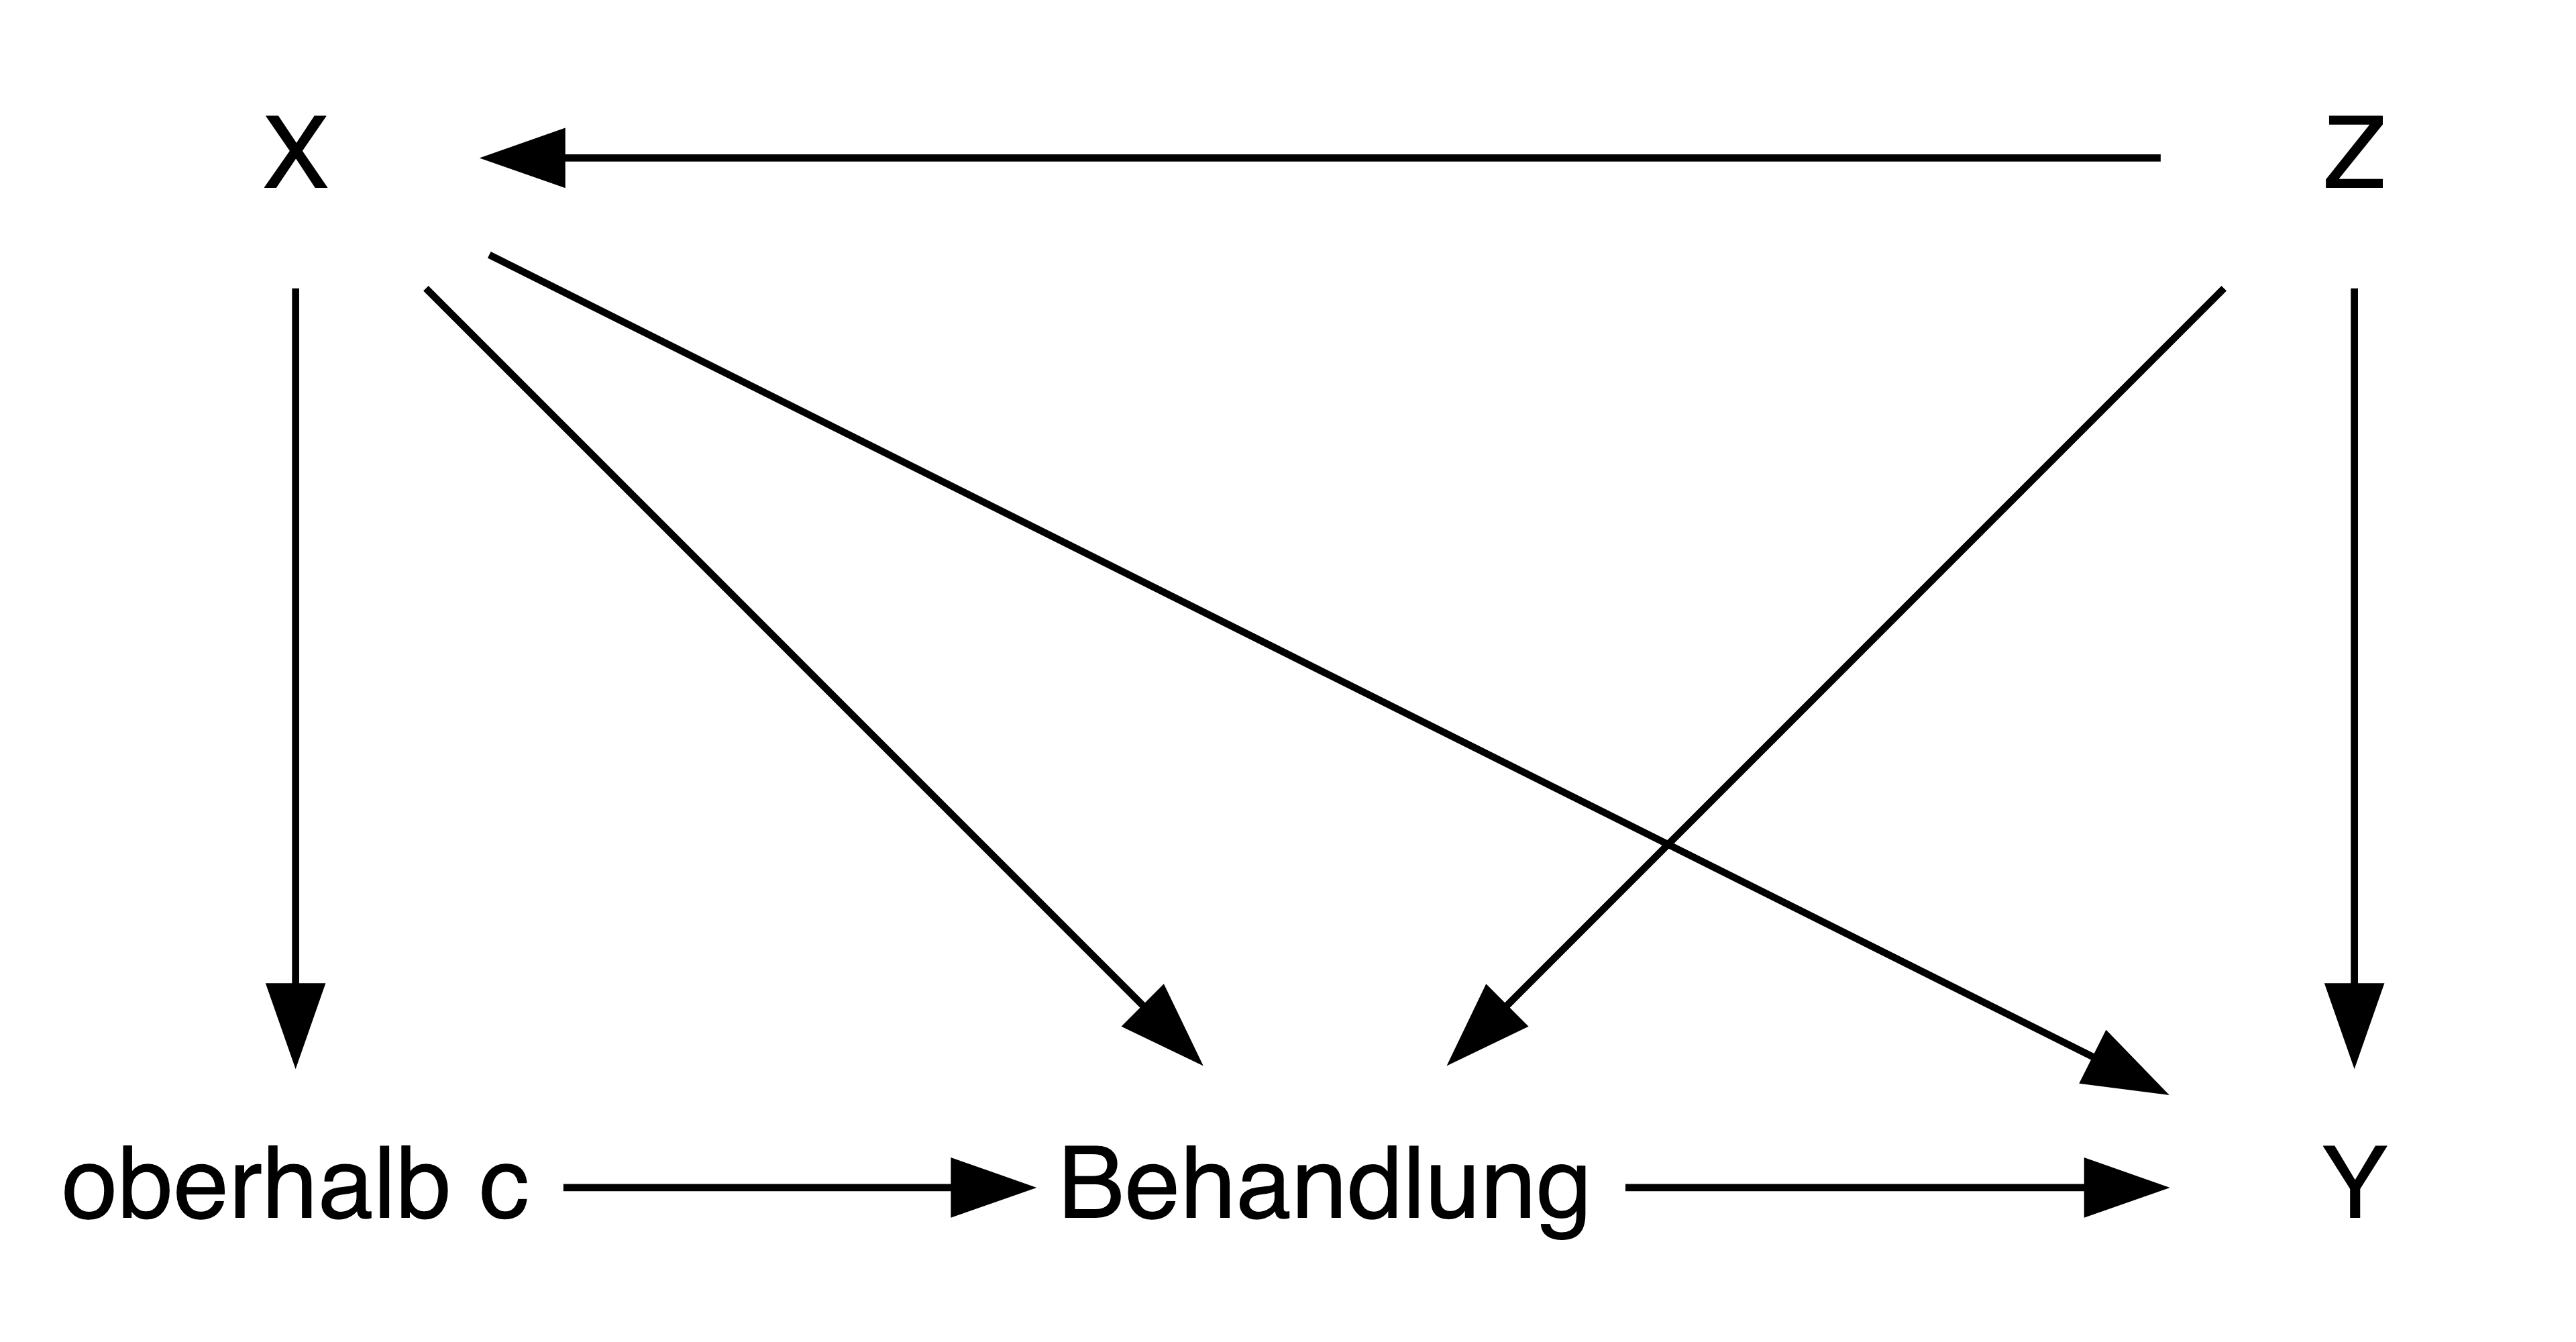
\includegraphics[width=5in,height=3in]{RDD_files/figure-latex/dot-figure-2.png}

}

\end{figure}

}

\caption{\label{fig-CDFRDD}Causal Diagram für FRDD}

\end{figure}

\hypertarget{case-study-protestantische-arbeitsethik}{%
\section{Case Study: Protestantische
Arbeitsethik}\label{case-study-protestantische-arbeitsethik}}

Die Studie \emph{Beyond Work Ethic: Religion, Individual, and Political
Preferences} (\textbf{BastenBetz2013?}) untersucht den Zusammenhang
zwischen Religion, individuellen Merkmalen und politischen Präferenzen.
Das Hauptaugenmerk ist die Rolle von Religiosität als Einflussfaktor auf
politische Einstellungen. Die Hypothese ist, das Religiosität eines
Individuums über den traditionellen Rahmen von Moralvorstellungen und
sozialen Normen hinaus auch politische Präferenzen beeinflusst. Diese
Theorie wird prominent von Max Weber (1930) vertreten, der argumentiert,
dass die protestantische Arbeitsethik einen entscheidenden Einfluss auf
die Entwicklung des Kapitalismus hatte. Laut Weber führte der
protestantische Glaube an harte Arbeit, ein sparsames Leben und
ethisches Verhalten zur einer verbreiteten ``Geisteshaltung'' , die den
wirtschaftlichen Erfolg förderte und den Aufstieg des Kapitalismus
begünstigte.

(\textbf{BastenBetz2013?}) nutzen Daten aus dem World Values Survey,

Sie analysieren insbesondere die Zusammenhänge zwischen Religiosität,
individuellen Merkmalen wie Geschlecht, Bildung und Einkommen sowie
politischen Präferenzen wie links-rechts-Ausrichtung, Einstellungen zur
Umverteilung und zur Einwanderung.

Die Ergebnisse der Studie zeigen, dass Religiosität tatsächlich einen
signifikanten Einfluss auf politische Präferenzen hat. Insbesondere
stellen die Autoren fest, dass religiöse Menschen tendenziell
konservativere Einstellungen haben und eher rechten politischen Parteien
zuneigen. Dieser Effekt bleibt auch nach Kontrolle anderer Faktoren wie
Bildung und Einkommen bestehen.

Darüber hinaus betonen die Autoren, dass der Zusammenhang zwischen
Religion und politischen Präferenzen nicht allein durch moralische Werte
erklärt werden kann. Sie argumentieren, dass religiöse Institutionen
auch eine soziale und politische Agenda verfolgen, die von den Gläubigen
internalisiert wird. Diese Agenda kann beispielsweise Positionen zu
Themen wie Abtreibung, gleichgeschlechtlicher Ehe, Einwanderung oder
Umweltschutz umfassen.

Zusammenfassend zeigt das Paper ``Beyond Work Ethic: Religion,
Individual, and Political Preferences'' von Christoph Basten und Frank
Betz, dass Religiosität einen Einfluss auf politische Präferenzen hat,
der über traditionelle Moralvorstellungen hinausgeht. Es deutet darauf
hin, dass religiöse Menschen eher konservative politische Ansichten
haben und dass religiöse Institutionen eine Rolle bei der Formulierung
dieser Ansichten spielen können.

\begin{Shaded}
\begin{Highlighting}[]
\FunctionTok{library}\NormalTok{(tidyverse)}
\FunctionTok{library}\NormalTok{(haven)}
\FunctionTok{library}\NormalTok{(vtable)}
\FunctionTok{library}\NormalTok{(rdrobust)}
\end{Highlighting}
\end{Shaded}

\begin{Shaded}
\begin{Highlighting}[]
\NormalTok{BastenBetz }\OtherTok{\textless{}{-}} \FunctionTok{read\_dta}\NormalTok{(}\StringTok{\textquotesingle{}BastenBetz.dta\textquotesingle{}}\NormalTok{)}
\end{Highlighting}
\end{Shaded}

\begin{Shaded}
\begin{Highlighting}[]
\CommentTok{\# Table 1}
\NormalTok{T1 }\OtherTok{\textless{}{-}}\NormalTok{ BastenBetz }\SpecialCharTok{\%\textgreater{}\%}
    \FunctionTok{filter}\NormalTok{(}\FunctionTok{abs}\NormalTok{(borderdis) }\SpecialCharTok{\textless{}} \FloatTok{5.0283684}\NormalTok{) }\SpecialCharTok{\%\textgreater{}\%}
    \FunctionTok{transmute}\NormalTok{(}
        \AttributeTok{group =} \FunctionTok{ifelse}\NormalTok{(vaud }\SpecialCharTok{==} \DecValTok{1}\NormalTok{, }\StringTok{"T"}\NormalTok{, }\StringTok{"C"}\NormalTok{),}
        \AttributeTok{prot1980s =}\NormalTok{ prot1980s }\SpecialCharTok{*} \DecValTok{100}\NormalTok{,}
        \AttributeTok{reineink =}\NormalTok{ reineink\_pc\_mean }\SpecialCharTok{*} \DecValTok{1000}\NormalTok{,}
\NormalTok{        noreligion1980s,}
\NormalTok{        altitude, }
\NormalTok{        pfl, }
\NormalTok{        pfr, }
\NormalTok{        pfi,}
        \AttributeTok{gini =}\NormalTok{ Ecoplan\_gini}
\NormalTok{    ) }\SpecialCharTok{\%\textgreater{}\%}
    \FunctionTok{group\_by}\NormalTok{(group) }\SpecialCharTok{\%\textgreater{}\%}
    \FunctionTok{summarise}\NormalTok{(}
      \FunctionTok{across}\NormalTok{(}\FunctionTok{everything}\NormalTok{(), }\FunctionTok{list}\NormalTok{(}\AttributeTok{Mean =}\NormalTok{ mean, }\AttributeTok{SD =}\NormalTok{ sd, }\AttributeTok{N =}\NormalTok{ length))}
\NormalTok{      ) }\SpecialCharTok{\%\textgreater{}\%}
    \FunctionTok{pivot\_longer}\NormalTok{(}
      \SpecialCharTok{{-}}\NormalTok{group, }
      \AttributeTok{names\_to =} \FunctionTok{c}\NormalTok{(}\StringTok{"variable"}\NormalTok{, }\StringTok{"statistic"}\NormalTok{), }
      \AttributeTok{names\_sep =} \StringTok{"\_"}
\NormalTok{    )}
\end{Highlighting}
\end{Shaded}

\begin{Shaded}
\begin{Highlighting}[]
\NormalTok{T1\_wider }\OtherTok{\textless{}{-}}\NormalTok{ T1 }\SpecialCharTok{\%\textgreater{}\%} 
    \FunctionTok{pivot\_wider}\NormalTok{(}
        \AttributeTok{names\_from =} \FunctionTok{c}\NormalTok{(}\StringTok{"group"}\NormalTok{, }\StringTok{"statistic"}\NormalTok{)}
\NormalTok{    )}
\end{Highlighting}
\end{Shaded}

\begin{Shaded}
\begin{Highlighting}[]
\NormalTok{T1\_wider }\SpecialCharTok{\%\textgreater{}\%}
  \FunctionTok{gt}\NormalTok{(}\AttributeTok{rowname\_col =} \StringTok{"Variable"}\NormalTok{) }\SpecialCharTok{\%\textgreater{}\%} 
  \FunctionTok{tab\_spanner\_delim}\NormalTok{(}
    \AttributeTok{delim =} \StringTok{"\_"}\NormalTok{,}
\NormalTok{  ) }\SpecialCharTok{\%\textgreater{}\%}
\NormalTok{ tabopts}
\end{Highlighting}
\end{Shaded}

\hypertarget{tbl-sumstat}{}
\begin{longtable}{lrrrrrr}
\caption{\label{tbl-sumstat}Datensatz \texttt{BastenBetz} -- Zusammenfassende Statistiken }\tabularnewline

\toprule
 & \multicolumn{3}{c}{C} & \multicolumn{3}{c}{T} \\ 
\cmidrule(lr){2-4} \cmidrule(lr){5-7}
variable & Mean & SD & N & Mean & SD & N \\ 
\midrule
prot1980s & $9.428$ & $5.695$ & $49$ & $83.245$ & $11.411$ & $84$ \\ 
reineink & $43,692.71$ & $3,369.175$ & $49$ & $47,253.272$ & $5,342.36$ & $84$ \\ 
noreligion1980s & $1.729$ & $1.499$ & $49$ & $2.95$ & $2.726$ & $84$ \\ 
altitude & $642.592$ & $120.23$ & $49$ & $639.607$ & $113.564$ & $84$ \\ 
pfl & $48.239$ & $4.774$ & $49$ & $39.508$ & $5.723$ & $84$ \\ 
pfr & $43.049$ & $2.634$ & $49$ & $39.19$ & $5.025$ & $84$ \\ 
pfi & $52.642$ & $2.94$ & $49$ & $47.086$ & $3.368$ & $84$ \\ 
gini & $0.302$ & $0.029$ & $49$ & $0.367$ & $0.052$ & $84$ \\ 
\bottomrule
\end{longtable}

Imbens und Kalyanaraman (2012) zeigen

\begin{Shaded}
\begin{Highlighting}[]
\NormalTok{bw\_selection }\OtherTok{\textless{}{-}} \FunctionTok{rdbwselect}\NormalTok{(}
  \AttributeTok{y =}\NormalTok{ BastenBetz}\SpecialCharTok{$}\NormalTok{pfl,}
  \AttributeTok{x =}\NormalTok{ BastenBetz}\SpecialCharTok{$}\NormalTok{borderdis,}
  \AttributeTok{fuzzy =}\NormalTok{ BastenBetz}\SpecialCharTok{$}\NormalTok{prot1980s, }
  \AttributeTok{bwselect =} \StringTok{"mserd"}\NormalTok{, }
  \AttributeTok{kernel =} \StringTok{"uniform"}\NormalTok{) }

\FunctionTok{summary}\NormalTok{(bw\_selection)}
\end{Highlighting}
\end{Shaded}

\begin{verbatim}
Call: rdbwselect

Number of Obs.                  509
BW type                       mserd
Kernel                      Uniform
VCE method                       NN

Number of Obs.                  127          382
Order est. (p)                    1            1
Order bias  (q)                   2            2
Unique Obs.                      97          261

=======================================================
                  BW est. (h)    BW bias (b)
            Left of c Right of c  Left of c Right of c
=======================================================
     mserd     5.078      5.078     10.905     10.905
=======================================================
\end{verbatim}

\begin{Shaded}
\begin{Highlighting}[]
\NormalTok{OB }\OtherTok{\textless{}{-}}\NormalTok{ bw\_selection}\SpecialCharTok{$}\NormalTok{bws[}\DecValTok{1}\NormalTok{]}
\end{Highlighting}
\end{Shaded}

\begin{Shaded}
\begin{Highlighting}[]
\CommentTok{\# Table 2: First stage results }
\CommentTok{\# (1) (close to the) Imbens and Kalyanaraman (2012) optimal BW of 5.01 reported in}
\CommentTok{\# the paper}
\NormalTok{FS1 }\OtherTok{\textless{}{-}} \FunctionTok{lm}\NormalTok{(}
  \AttributeTok{formula =}\NormalTok{ prot1980s }\SpecialCharTok{\textasciitilde{}}\NormalTok{ vaud }\SpecialCharTok{+}\NormalTok{ borderdis }\SpecialCharTok{+}\NormalTok{ vaud }\SpecialCharTok{*}\NormalTok{ borderdis, }
  \AttributeTok{data =}\NormalTok{ BastenBetz }\SpecialCharTok{\%\textgreater{}\%} \FunctionTok{filter}\NormalTok{(}\FunctionTok{abs}\NormalTok{(borderdis) }\SpecialCharTok{\textless{}}\NormalTok{ OB)}
\NormalTok{  )}

\CommentTok{\# (2) Constant BW: 10}
\NormalTok{FS2 }\OtherTok{\textless{}{-}} \FunctionTok{lm}\NormalTok{(}
  \AttributeTok{formula =}\NormalTok{ prot1980s }\SpecialCharTok{\textasciitilde{}}\NormalTok{ vaud }\SpecialCharTok{+}\NormalTok{ borderdis }\SpecialCharTok{+}\NormalTok{ vaud }\SpecialCharTok{*}\NormalTok{ borderdis, }
  \AttributeTok{data =}\NormalTok{ BastenBetz }\SpecialCharTok{\%\textgreater{}\%} \FunctionTok{filter}\NormalTok{(}\FunctionTok{abs}\NormalTok{(borderdis) }\SpecialCharTok{\textless{}} \DecValTok{10}\NormalTok{)}
\NormalTok{  )}

\CommentTok{\# (3)  Constant BW: 20}
\NormalTok{FS3 }\OtherTok{\textless{}{-}} \FunctionTok{lm}\NormalTok{(}
  \AttributeTok{formula =}\NormalTok{ prot1980s }\SpecialCharTok{\textasciitilde{}}\NormalTok{ vaud }\SpecialCharTok{+}\NormalTok{ borderdis }\SpecialCharTok{+}\NormalTok{ vaud }\SpecialCharTok{*}\NormalTok{ borderdis, }
  \AttributeTok{data =}\NormalTok{ BastenBetz }\SpecialCharTok{\%\textgreater{}\%} \FunctionTok{filter}\NormalTok{(}\FunctionTok{abs}\NormalTok{(borderdis) }\SpecialCharTok{\textless{}} \DecValTok{20}\NormalTok{)}
\NormalTok{  )}
\end{Highlighting}
\end{Shaded}

\begin{Shaded}
\begin{Highlighting}[]
\NormalTok{modelsummary}\SpecialCharTok{::}\FunctionTok{modelsummary}\NormalTok{(}
  \FunctionTok{list}\NormalTok{(FS1, FS2, FS3), }
  \AttributeTok{vcov =} \StringTok{"HC1"}\NormalTok{, }\AttributeTok{stars =}\NormalTok{ T, }\AttributeTok{gof\_map =} \StringTok{"nobs"}\NormalTok{, }\AttributeTok{output =} \StringTok{"gt"}
\NormalTok{) }\SpecialCharTok{\%\textgreater{}\%}
  \FunctionTok{tabopts}\NormalTok{()}
\end{Highlighting}
\end{Shaded}

\setlength{\LTpost}{0mm}
\begin{longtable*}{lccc}
\toprule
  & (1) & (2) & (3) \\ 
\midrule
(Intercept) & 0.134*** & 0.100*** & 0.103*** \\ 
 & (0.017) & (0.013) & (0.010) \\ 
vaud & 0.671*** & 0.726*** & 0.756*** \\ 
 & (0.034) & (0.022) & (0.018) \\ 
borderdis & 0.017** & 0.001 & 0.001 \\ 
 & (0.006) & (0.003) & (0.001) \\ 
vaud × borderdis & -0.006 & -0.001 & -0.009*** \\ 
 & (0.012) & (0.005) & (0.003) \\ 
Num.Obs. & 133 & 207 & 312 \\ 
\bottomrule
\end{longtable*}
\begin{minipage}{\linewidth}
+ p < 0.1, * p < 0.05, ** p < 0.01, *** p < 0.001\\
\end{minipage}

\begin{Shaded}
\begin{Highlighting}[]
\CommentTok{\# Figure 3}
\NormalTok{rdrobust}\SpecialCharTok{::}\FunctionTok{rdplot}\NormalTok{(}\AttributeTok{y =}\NormalTok{ BastenBetz}\SpecialCharTok{$}\NormalTok{prot1980s, }
                 \AttributeTok{x =}\NormalTok{ BastenBetz}\SpecialCharTok{$}\NormalTok{borderdis, }
                 \AttributeTok{h =} \FunctionTok{c}\NormalTok{(OB, OB), }
                 \AttributeTok{p =} \DecValTok{1}\NormalTok{, }
                 \AttributeTok{nbins =} \FunctionTok{c}\NormalTok{(}\DecValTok{6}\NormalTok{, }\DecValTok{14}\NormalTok{), }
                 \AttributeTok{masspoints =} \StringTok{"off"}\NormalTok{)}
\NormalTok{rdrobust}\SpecialCharTok{::}\FunctionTok{rdplot}\NormalTok{(}\AttributeTok{y =}\NormalTok{ BastenBetz}\SpecialCharTok{$}\NormalTok{prot1980s, }
                 \AttributeTok{x =}\NormalTok{ BastenBetz}\SpecialCharTok{$}\NormalTok{borderdis, }
                 \AttributeTok{h =} \FunctionTok{c}\NormalTok{(}\DecValTok{10}\NormalTok{, }\DecValTok{10}\NormalTok{), }
                 \AttributeTok{p =} \DecValTok{1}\NormalTok{, }
                 \AttributeTok{nbins =} \FunctionTok{c}\NormalTok{(}\DecValTok{6}\NormalTok{, }\DecValTok{14}\NormalTok{),}
                  \AttributeTok{masspoints =} \StringTok{"off"}\NormalTok{)}
\NormalTok{rdrobust}\SpecialCharTok{::}\FunctionTok{rdplot}\NormalTok{(}\AttributeTok{y =}\NormalTok{ BastenBetz}\SpecialCharTok{$}\NormalTok{prot1980s, }
                 \AttributeTok{x =}\NormalTok{ BastenBetz}\SpecialCharTok{$}\NormalTok{borderdis, }
                 \AttributeTok{h =} \FunctionTok{c}\NormalTok{(}\DecValTok{20}\NormalTok{, }\DecValTok{20}\NormalTok{), }
                 \AttributeTok{p =} \DecValTok{1}\NormalTok{, }
                 \AttributeTok{nbins =} \FunctionTok{c}\NormalTok{(}\DecValTok{6}\NormalTok{, }\DecValTok{14}\NormalTok{),}
                  \AttributeTok{masspoints =} \StringTok{"off"}\NormalTok{)}
\NormalTok{rdrobust}\SpecialCharTok{::}\FunctionTok{rdplot}\NormalTok{(}\AttributeTok{y =}\NormalTok{ BastenBetz}\SpecialCharTok{$}\NormalTok{prot1980s, }
                 \AttributeTok{x =}\NormalTok{ BastenBetz}\SpecialCharTok{$}\NormalTok{borderdis, }
                 \AttributeTok{p =} \DecValTok{1}\NormalTok{, }
                 \AttributeTok{nbins =} \FunctionTok{c}\NormalTok{(}\DecValTok{6}\NormalTok{, }\DecValTok{14}\NormalTok{),}
                 \AttributeTok{masspoints =} \StringTok{"off"}\NormalTok{)}
\end{Highlighting}
\end{Shaded}

\begin{figure}

\begin{minipage}[t]{0.50\linewidth}

{\centering 

\raisebox{-\height}{

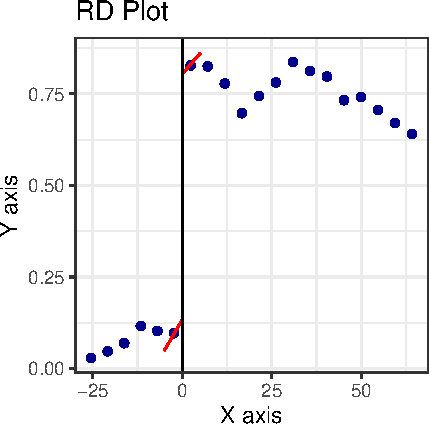
\includegraphics{RDD_files/figure-pdf/unnamed-chunk-26-1.pdf}

}

}

\end{minipage}%
%
\begin{minipage}[t]{0.50\linewidth}

{\centering 

\raisebox{-\height}{

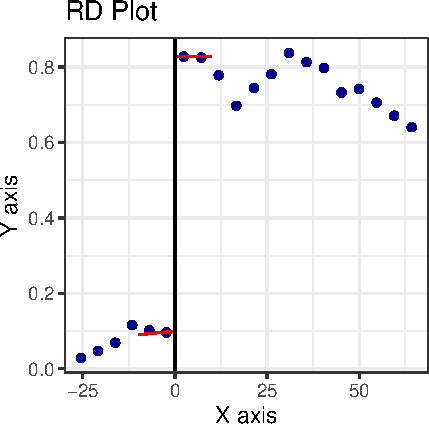
\includegraphics{RDD_files/figure-pdf/unnamed-chunk-26-2.pdf}

}

}

\end{minipage}%
\newline
\begin{minipage}[t]{0.50\linewidth}

{\centering 

\raisebox{-\height}{

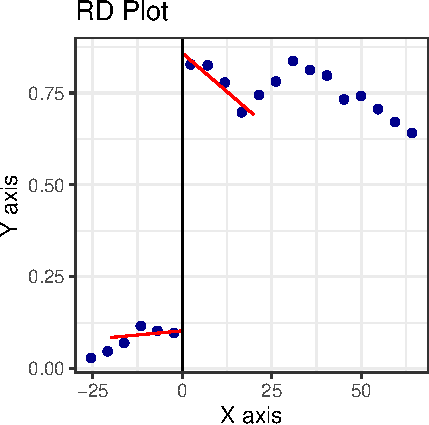
\includegraphics{RDD_files/figure-pdf/unnamed-chunk-26-3.pdf}

}

}

\end{minipage}%
%
\begin{minipage}[t]{0.50\linewidth}

{\centering 

\raisebox{-\height}{

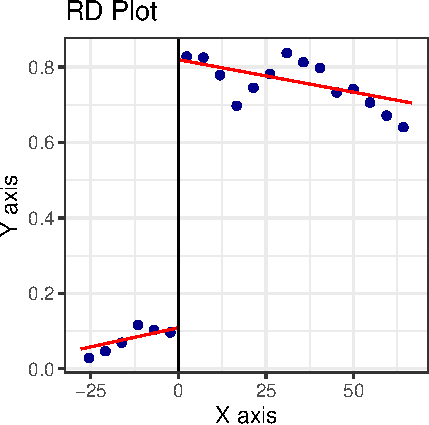
\includegraphics{RDD_files/figure-pdf/unnamed-chunk-26-4.pdf}

}

}

\end{minipage}%

\end{figure}

\bookmarksetup{startatroot}

\hypertarget{summary}{%
\chapter{Summary}\label{summary}}

In summary, this book has no content whatsoever.

\begin{Shaded}
\begin{Highlighting}[]
\DecValTok{1} \SpecialCharTok{+} \DecValTok{1}
\end{Highlighting}
\end{Shaded}

\begin{verbatim}
[1] 2
\end{verbatim}

\bookmarksetup{startatroot}

\hypertarget{demo}{%
\chapter{Demo}\label{demo}}

\hypertarget{background}{%
\section{Background}\label{background}}

The purpose of this document is to explore how WebR can be embedded in a
Quarto Document for the purposes of teaching \emph{R}.

\begin{itemize}
\tightlist
\item
  WebR Website: \url{https://docs.r-wasm.org/webr/latest/}
\item
  WebR GitHub: \url{https://github.com/r-wasm/webr/}
\end{itemize}

\hypertarget{setup}{%
\section{Setup}\label{setup}}

See the \url{https://github.com/coatless-r-n-d/webR-quarto-demos} for
source.

\hypertarget{exploration}{%
\section{Exploration}\label{exploration}}

Next, let's look at a few features of the language

\hypertarget{linear-regression}{%
\subsection{Linear Regression}\label{linear-regression}}

We'll first start with the WebR team's demo example or the statistician
way of saying, ``Hello world!''\ldots{} Aka linear regression:

R lädt. Etwas Geduld bitte\ldots{}

\hypertarget{webr-editor-1}{}

\hypertarget{webr-code-output-1}{}

\hypertarget{retrieving-prior-objects}{%
\subsection{Retrieving prior objects}\label{retrieving-prior-objects}}

Each WebR cell appears to be connected to each other. Thus, we can
access the \texttt{fit} outcome:

R lädt. Etwas Geduld bitte\ldots{}

\hypertarget{webr-editor-2}{}

\hypertarget{webr-code-output-2}{}

R lädt. Etwas Geduld bitte\ldots{}

\hypertarget{webr-editor-3}{}

\hypertarget{webr-code-output-3}{}

\hypertarget{mixing-active-and-non-active-r-code}{%
\subsection{\texorpdfstring{Mixing active and non-active \emph{R}
code}{Mixing active and non-active R code}}\label{mixing-active-and-non-active-r-code}}

For \emph{if-else} statements, we have:

\begin{Shaded}
\begin{Highlighting}[]
\ControlFlowTok{if}\NormalTok{ (...) \{}
  \CommentTok{\# Statements for TRUE}
\NormalTok{\} }\ControlFlowTok{else}\NormalTok{ \{}
  \CommentTok{\# Statements for FALSE}
\NormalTok{\}}
\end{Highlighting}
\end{Shaded}

\begin{itemize}
\tightlist
\item
  \texttt{...} denotes a condition (either \texttt{TRUE} or
  \texttt{FALSE})
\item
  If \texttt{TRUE}, then run the statements inside \texttt{\{\}}
\item
  Else, \texttt{FALSE}, carry on with your day.
\end{itemize}

How could we modify \texttt{temperature} to have the \texttt{if}
statement print \texttt{"Hot!"}?

R lädt. Etwas Geduld bitte\ldots{}

\hypertarget{webr-editor-4}{}

\hypertarget{webr-code-output-4}{}

\hypertarget{summarize-data}{%
\subsection{Summarize Data}\label{summarize-data}}

Glancing at data frames yields:

R lädt. Etwas Geduld bitte\ldots{}

\hypertarget{webr-editor-5}{}

\hypertarget{webr-code-output-5}{}

\hypertarget{errors-and-warnings}{%
\subsection{Errors and Warnings}\label{errors-and-warnings}}

R lädt. Etwas Geduld bitte\ldots{}

\hypertarget{webr-editor-6}{}

\hypertarget{webr-code-output-6}{}

R lädt. Etwas Geduld bitte\ldots{}

\hypertarget{webr-editor-7}{}

\hypertarget{webr-code-output-7}{}

\hypertarget{base-graphics}{%
\subsection{Base graphics}\label{base-graphics}}

Graphing with base R

R lädt. Etwas Geduld bitte\ldots{}

\hypertarget{webr-editor-8}{}

\hypertarget{webr-code-output-8}{}

More advanced base R graphing\ldots{}

R lädt. Etwas Geduld bitte\ldots{}

\hypertarget{webr-editor-9}{}

\hypertarget{webr-code-output-9}{}

\hypertarget{ggplot2-graphics}{%
\subsection{ggplot2 Graphics}\label{ggplot2-graphics}}

Next, we look at using \texttt{ggplot2} graphics. By default, the
\texttt{ggplot2} package is not available as it is \emph{dependency}
heavy.

R lädt. Etwas Geduld bitte\ldots{}

\hypertarget{webr-editor-10}{}

\hypertarget{webr-code-output-10}{}

\bookmarksetup{startatroot}

\hypertarget{references}{%
\chapter*{References}\label{references}}
\addcontentsline{toc}{chapter}{References}

\markboth{References}{References}

\hypertarget{refs}{}
\begin{CSLReferences}{1}{0}
\leavevmode\vadjust pre{\hypertarget{ref-AngristPischke2010}{}}%
Angrist, Joshua D, und Jörn-Steffen Pischke. 2010. {„The credibility
revolution in empirical economics: How better research design is taking
the con out of econometrics``}. \emph{Journal of economic perspectives}
24 (2): 3--30.

\leavevmode\vadjust pre{\hypertarget{ref-ImbensLemieux2008}{}}%
Imbens, G. W., und Thomas Lemieux. 2008. {„Regression discontinuity
designs: A guide to practice``}. \emph{Journal of econometrics} 142 (2):
615--35.

\leavevmode\vadjust pre{\hypertarget{ref-ImbensKalyanaraman2012}{}}%
Imbens, Guido, und Karthik Kalyanaraman. 2012. {„Optimal bandwidth
choice for the regression discontinuity estimator``}. \emph{The Review
of economic studies} 79 (3): 933--59.

\leavevmode\vadjust pre{\hypertarget{ref-Lee2008}{}}%
Lee, David S. 2008. {„Randomized experiments from non-random selection
in US House elections``}. \emph{Journal of Econometrics} 142 (2):
675--97.

\end{CSLReferences}



\end{document}
